\documentclass[aspectratio=169,12pt]{beamer}
\usetheme{Madrid}
\usecolortheme{dolphin}
\usefonttheme{professionalfonts}
\setbeamertemplate{navigation symbols}{}
\setbeamertemplate{footline}{}

\usepackage[T1]{fontenc}
\usepackage[utf8]{inputenc}
\usepackage{graphicx}
\usepackage{amsmath,amssymb}
\usepackage{hyperref}
\usepackage{siunitx}
\usepackage{physics}

\begin{document}

\title[Chapter 2]{Chapitre 2: Vecteurs, qubit et superposition}
\author{JAMOTTE Maxime, SCHOONEN Cédric}
\institute{Digital Learning Hub}
\date{}

\begin{frame}
  \titlepage
\end{frame}

\begin{frame}{Objectifs du chapitre 2}
  \begin{enumerate}
    \item Vecteurs\\~\\
    \item Produit scalaire\\~\\
    \item Qubit, superposition d'états et vecteurs
  \end{enumerate}
\end{frame}

\begin{frame}{Vecteurs}
  {%
    \setbeamercolor{itemize/enumerate body}{fg=gray!60}
    \setbeamercolor{itemize item}{fg=gray!60}
    \setbeamercolor{alerted text}{fg=black}
    \begin{columns}[T]
      \begin{column}{0.55\textwidth}
        \begin{itemize}[<+-| alert@+>]
          \setlength{\itemsep}{0.6em}
          \item Définition d'un vecteur
          \item Addition de vecteurs
          \item Multiplication d'un vecteur par une constante
        \end{itemize}
        \bigskip
        \only<1>{\[
          \vec r = \begin{pmatrix} a \\ b \end{pmatrix}
        \]}
        \only<2>{\[
          \vec r + \vec p = 
          \begin{pmatrix} a \\ b \end{pmatrix} +
          \begin{pmatrix} c \\ d \end{pmatrix} =
          \begin{pmatrix} a+c \\ b+d \end{pmatrix}
        \]}
        \only<3>{\[
          \lambda \begin{pmatrix} a \\ b \end{pmatrix} =
          \begin{pmatrix} \lambda a \\ \lambda b \end{pmatrix}
        \]}
      \end{column}
      \begin{column}{0.4\textwidth}
        \centering
        \only<1>{\includegraphics[width=\linewidth]{figures/vecteur.png}}
        \only<2>{\includegraphics[width=\linewidth]{figures/add_vecteurs.png}}
        \only<3->{\includegraphics[width=\linewidth]{figures/multiplication_nombre.png}}
      \end{column}
    \end{columns}
  }
\end{frame}

\begin{frame}{Produit scalaire}
  \begin{columns}[T]
    \begin{column}{0.6\textwidth}
      \begin{itemize}[<+->]
        \setlength{\itemsep}{0.6em}
        \item La probabilité d'obtenir un résultat de mesure vient (en gros) d'une comparaison de deux états quantiques.
        \item Cette comparaison se traduit par un produit scalaire entre leurs vecteurs associés.
        $$\vec r \cdot \vec p = \begin{pmatrix} a & b \end{pmatrix} \begin{pmatrix} c \\ d \end{pmatrix} = ac+bd$$
        \item Lien avec l'angle: $\vec r \cdot \vec p = \norm{\vec r}\norm{\vec p}\cos(\theta)$.
      \end{itemize}
    \end{column}
    \begin{column}{0.35\textwidth}
      \centering
      \includegraphics[width=\linewidth]{figures/proj.png}
    \end{column}
  \end{columns}
\end{frame}

\begin{frame}{Qubit}
  \begin{itemize}[<+->]
    \setlength{\itemsep}{0.6em}
    %\item Electron autour du noyau: infinité de positions possibles.
    \item L'électron passe à travers les fentes du haut ($H$) et du bas ($B$) en même temps.% $\ket{\psi_e^{}} = \alpha \ket{H} + \beta \ket{B}$.
      \only<1->{%
        \vspace{0.5em}
        \begin{center}
          \begin{minipage}{0.42\textwidth}
            \centering
            \includegraphics[width=0.6\linewidth]{figures/fente_Young.png}
          \end{minipage}\hfill
          \begin{minipage}{0.42\textwidth}
            \centering
            \only<2->{\includegraphics[width=0.6\linewidth]{figures/bohr_model.png}}
          \end{minipage}
        \end{center}
      }
    \item Certains systèmes physiques ont des niveaux discrets d'énergie (au lieu de la position).
    \item \textbf{Qubit} (= bit quantique) = système quantique à 2 niveaux, notés $\ket 0$ et $\ket 1$.
  \end{itemize}
\end{frame}

\begin{frame}{Superposition d'états et vecteurs}
  \begin{columns}[T]
    \begin{column}{0.65\textwidth}
      \begin{itemize}[<+->]
        \item Un qubit peut être dans $\ket 0$, $\ket 1$ ou toute \textbf{superposition} des deux: $\alpha \ket 0 + \beta \ket 1$.
        \item Superposition = combinaison linéaire d'états.
        \item \textbf{Postulat} : les états quantiques forment un espace vectoriel (espace de Hilbert). Une combinaison linéaire d'états est aussi un état.
        \item L'état superposé $\ket {\psi} = \alpha \ket 0 + \beta \ket 1$, s'écrit $\begin{pmatrix} \alpha \\ \beta \end{pmatrix}$,\\~\\
        \item Chaque \textbf{qubit} est identifiable à la \textbf{direction} de son vecteur.
        \item Si deux vecteurs ont la \textbf{même direction} ($\theta = 0$), leurs qubits occupent le \textbf{même état}.
        %\item Probabilités de mesure : $P(\ket 0)=|\alpha|^2$, $P(\ket 1)=|\beta|^2$,
        %$$ \Longrightarrow  |\alpha|^2 + |\beta|^2 = 1$$
      \end{itemize}
    \end{column}
    \begin{column}{0.35\textwidth}
      \vspace{2em}
      \centering
      $\ket 0 = \begin{pmatrix}1 \\ 0\end{pmatrix}$ et $\ket 1 = \begin{pmatrix}0 \\ 1\end{pmatrix}$\\~\\~\\
      \only<4->{\includegraphics[width=0.8\textwidth]{figures/ket_base.png}}
    \end{column}
  \end{columns}
\end{frame}

\begin{frame}{Fin du chapitre 2}
  \begin{enumerate}
    \item Vecteurs\\~\\
    \item Produit scalaire\\~\\
    \item Qubit, superposition d'états et vecteurs
  \end{enumerate}
\end{frame}

\end{document}
